\chapter{Model Independent Study}
\section{$S_b$ Distribution}
The $S_b$ is defined as $S_b \equiv q^2/m^2_B$, where $q^2$ is the squared magnitude of the four-momentum transferred from the B meson to the neutrino pairs, and the $m_B$ is the mass of B meson.  Instead make a requirement on signal side candidate($K^*$) momentum, which is highly correlated to the $S_b$, we keep the full $S_b$ spectrum and provide the model-independent study bin-by-bin on $S_b$ spectrum. In this study, we perform the bin-by-bin optimization and calculate the partial branching fractions($\Delta \mathcal{B}$) in intervals of $S_b = 0.1$. With the full spectrum study, we have the opportunity to probe the hint of new physics. The $S_b$ distribution shown in Fig. \ref{fig:sb}.
    \begin{figure}[ht]
	\centering
	\subfigure[$K^{\pm}$ mode.]{
		\includegraphics[width=0.45\textwidth]{bin_by_bin_study_figure/knunu/sbcm_1025_1.eps}
		\label{ksb}
	}
	\subfigure[$K^{*\pm} \rightarrow K^\pm \pi^0$ mode.]{
		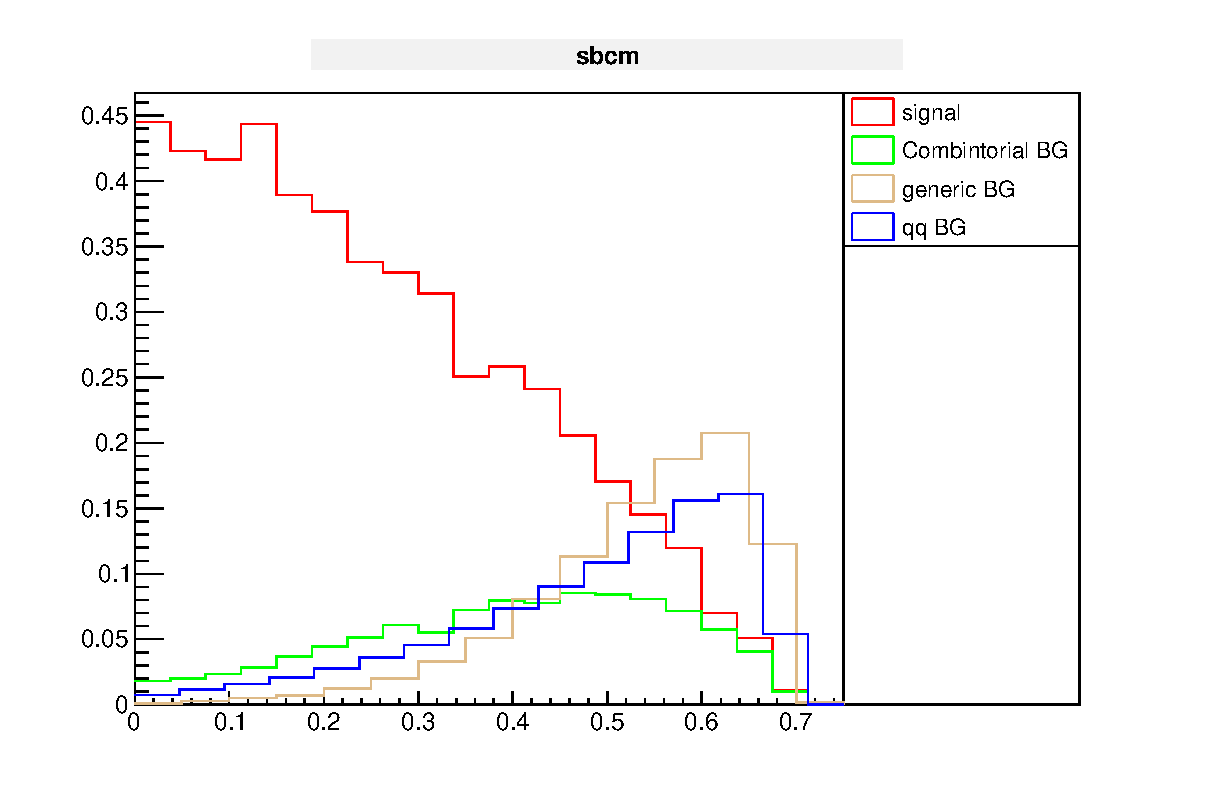
\includegraphics[width=0.45\textwidth]{bin_by_bin_study_figure/kstar1/sbcm_1025_kstar1.eps}
		\label{kpi0sb}
	}
	\subfigure[$K^{*\pm} \rightarrow K_s \pi^\pm$ mode.]{
		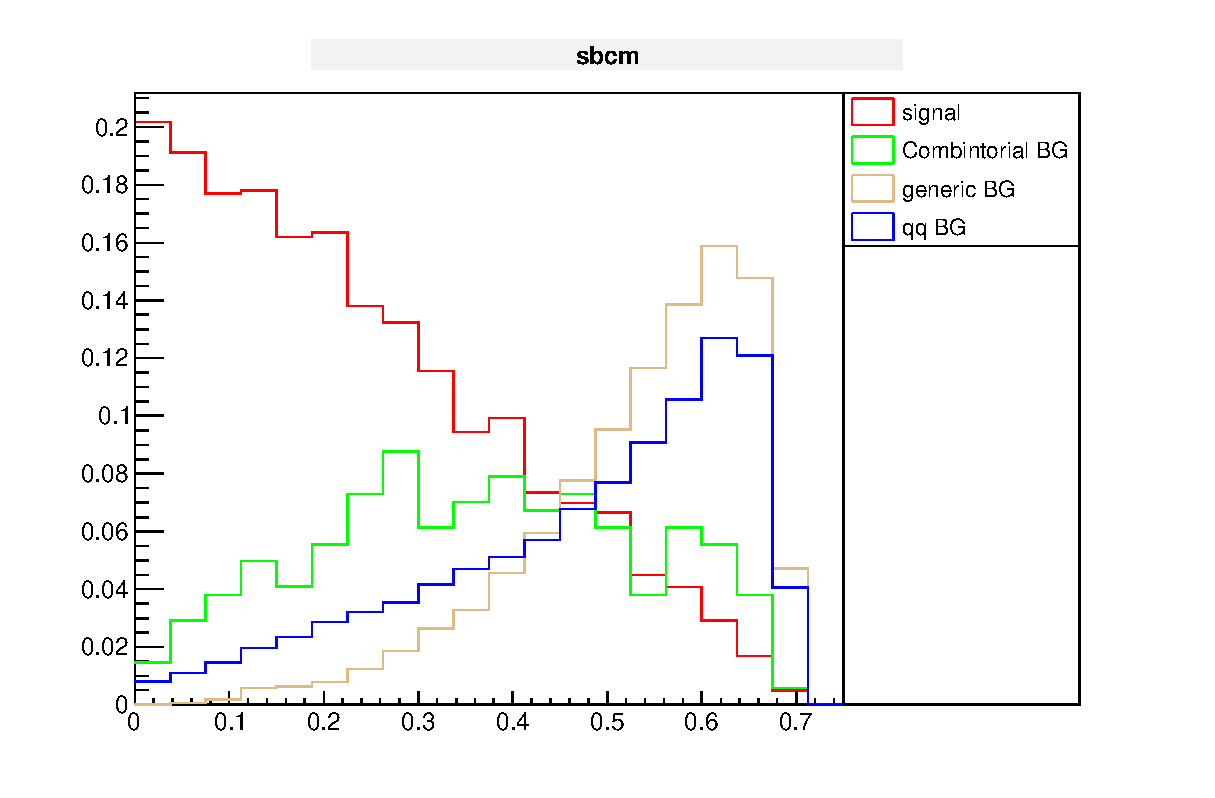
\includegraphics[width=0.45\textwidth]{bin_by_bin_study_figure/kstar2/sbcm_1025_112.eps}
		\label{kspisb}
	}
    \subfigure[$K^{*0}$ mode.]{
		\includegraphics[width=0.45\textwidth]{bin_by_bin_study_figure/k0/sbcm_1025_1.eps}
		\label{k0sb}
	}
    \subfigure[$K_s$ mode.]{
		\includegraphics[width=0.45\textwidth]{bin_by_bin_study_figure/kshort/sbcm_1025_1.eps}
		\label{kssb}
	}
\caption{$S_b$ distribution for each mode. Red represent signal, green represent the combintorial background,  brown represent the generic background and blue represent continuum background.}
\label{fig:sb}	
\end{figure}
\section{Neural-Network training}
In order to do the further separation between signal and background bin-by-bin, the powerful neural-network based multivariate analysis package Neurobayes is used. In this study, we use two kind of variables to training twice. One kind of variables is aiming to reduce the generic background; the other kind is shape variable from KSFW(Kakuno san's super fox-wolfram)\cite{ref:Lee2003} \cite{ref:fox1978}, there are 23 variables in total. 
\subsection{Training result} 
For the first kind of training, which is aiming to get rid of the generic background, we use generic MC sample as the background candidate, signal correct reconstruct MC sample as the signal candidate.The variables we use in first kind of NB training are list in table \ref{t:nbvlike_variables}, some of the variables list in table are based on Sebastian Neubauer's study~\cite{ref:Neubauer2011}. For the second kind of training(KSFW variables), we use continuum MC sample as the background candidate, signal correct reconstruct MC sample as the signal candidate.The training result with the table \ref{t:nbvlike_variables} for each mode is shown in Fig. \ref{fig:nbvlike}, The training result with KSFW variables is shown in Fig. \ref{fig:nbksfw}.
\begin{table}[ht]
\small
\begin{center}
\begin{tabular}{ |p{3cm}||p{10cm}|  }
 \hline
 cut& Description \\
 \hline
 \hline
  $B{\rm{tag}}\Delta E$   &  $\Delta E$ of Btag candidate.    \\
 \hline
 $B{\rm{tag}}M_{\rm{bc}}$   &  $M_{\rm{bc}}$ of Btag candidate.   \\
 \hline
 n\_ trackAll    & Number of additional track without any cuts.(i.e. no restrict on dr, dz and $P_T$ )  \\
  \hline
 n\_ pi0all    & Number of additional $\pi_0$ without any cuts.(no restrict on momentum )  \\
 \hline
 cosMEcm & Angle between the missing momentum and the whole event in the center of mass rest frame.\\
 \hline
 cos$\theta_{\rm{k}}$& Angle between signal candidate and Beam-pipe in lab frame.\\
 \hline
B$\Delta$dz& The different between the mean $|dz|$ of tag-side B signal condidate.  \\
 \hline
B$\Delta$dzsign& The significance of B$\Delta$dz.\\
\hline
 SumeclInMMdDir& The total enery measured by the calorimeter in a small cone around the direction of the missing-momentum.\\
 \hline
  $log(\rm{o_{tag}})$ & continuous suppression $NB_{\rm{out}}$\\
 \hline
RatiotoOthertype & the ratio of this BTag candidates NBout and the best of the other type if there is one.\\
 \hline
RatiotoSecondBest & the ratio of this BTag candidates NBout to the second best of this type if there is one.\\
 \hline
  $K^*$ mass   &  The invariant mass of $K^{*}$ candidate.    \\
 \hline
  $K^*$ child1 mass   &  The invariant mass of $K^{*}$ candidate first child.    \\
 \hline
  $K^*$ child2 mass   &  The invariant mass of $K^{*}$ candidate second child.    \\
 \hline
  Ddecay   &  Decay hashes of the tag-side D meson    \\
 \hline
  Tag\_expid   &  Experiment ID    \\
 \hline
\end{tabular}

\caption{The variables use in first kind of NB training, which is aiming to reduce the generic background. } \label{t:nbvlike_variables}
\end{center}
\end{table}

   \begin{figure}[ht]
	\centering
	\subfigure[$K^{\pm}$ mode.]{
		\includegraphics[width=0.45\textwidth]{bin_by_bin_study_figure/knunu/nb_vlike_1025_1.eps}
		\label{knbvlike}
	}
	\subfigure[$K^{*\pm} \rightarrow K^\pm \pi^0$ mode.]{
		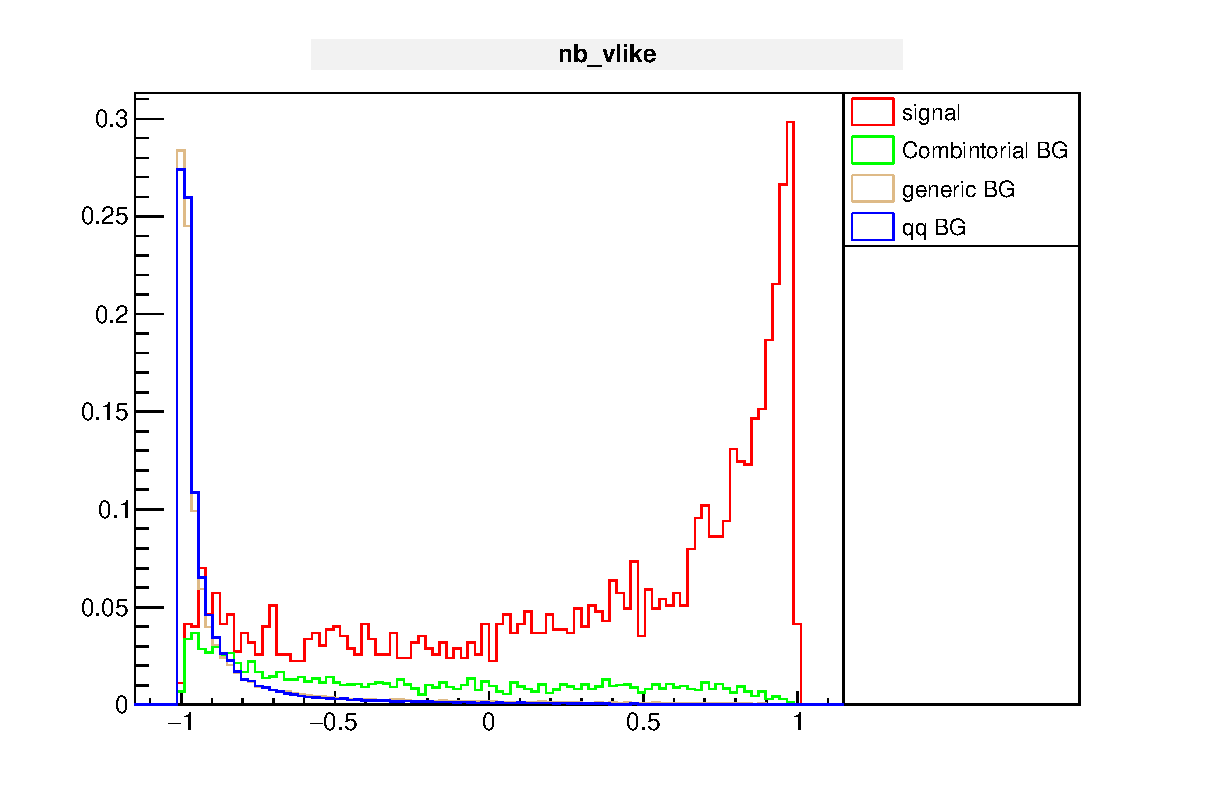
\includegraphics[width=0.45\textwidth]{bin_by_bin_study_figure/kstar1/nb_vlike_1025_kstar1.eps}
		\label{kpi0nbvlike}
	}
	\subfigure[$K^{*\pm} \rightarrow K_s \pi^\pm$ mode.]{
		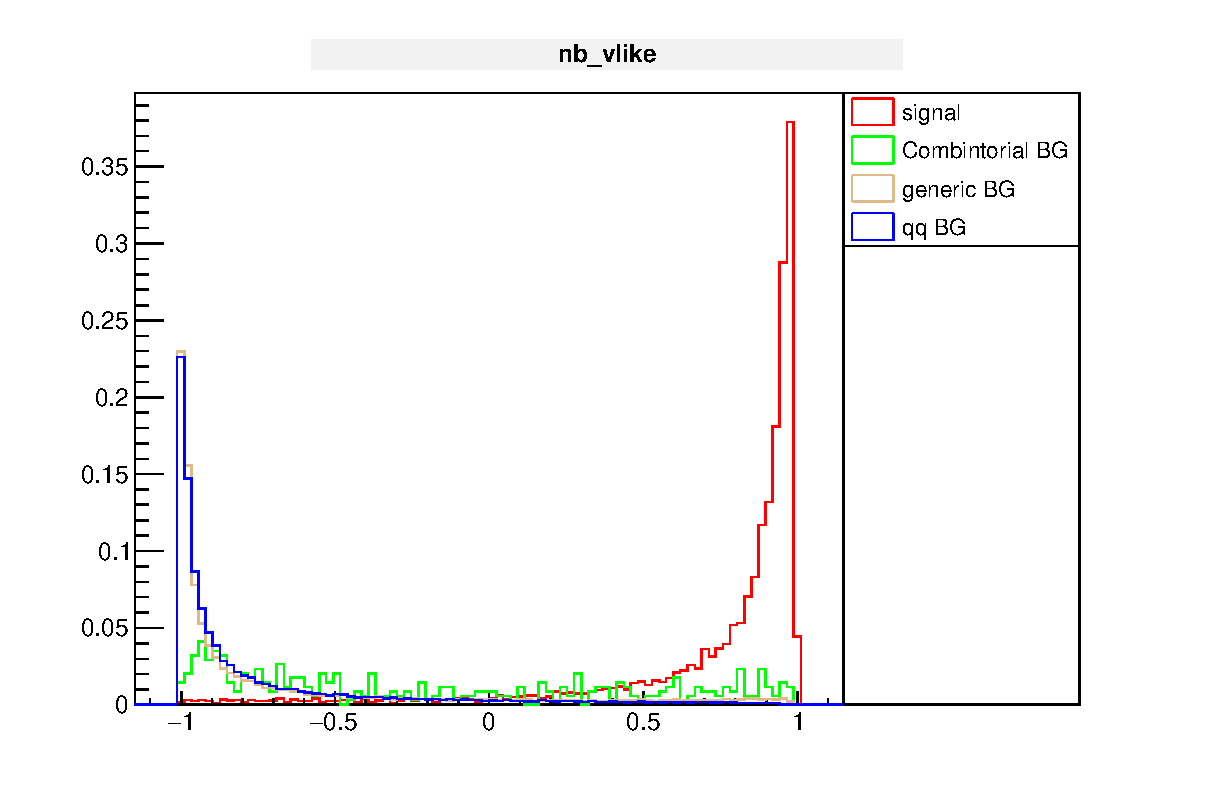
\includegraphics[width=0.45\textwidth]{bin_by_bin_study_figure/kstar2/nb_vlike_1025_112.eps}
		\label{kspinbvlike}
	}
    \subfigure[$K^{*0}$ mode.]{
		\includegraphics[width=0.45\textwidth]{bin_by_bin_study_figure/k0/nb_vlike_1025_1.eps}
		\label{k0nbvlike}
	}
    \subfigure[$K_s$ mode.]{
		\includegraphics[width=0.45\textwidth]{bin_by_bin_study_figure/kshort/nb_vlike_1025_1.eps}
		\label{ksnbvlike}
	}
\caption{Neurobayes output with variables list in table \ref{t:nbvlike_variables} for each mode. Red line represent signal, green line represent the combinatorial background,  brown line represent the generic background and blue line represent continuum background.}
\label{fig:nbvlike}	
\end{figure}

   \begin{figure}[ht]
	\centering
	\subfigure[$K^{\pm}$ mode.]{
		\includegraphics[width=0.45\textwidth]{bin_by_bin_study_figure/knunu/nb_ksfw_1025_1.eps}
		\label{knbksfw}
	}
	\subfigure[$K^{*\pm} \rightarrow K^\pm \pi^0$ mode.]{
		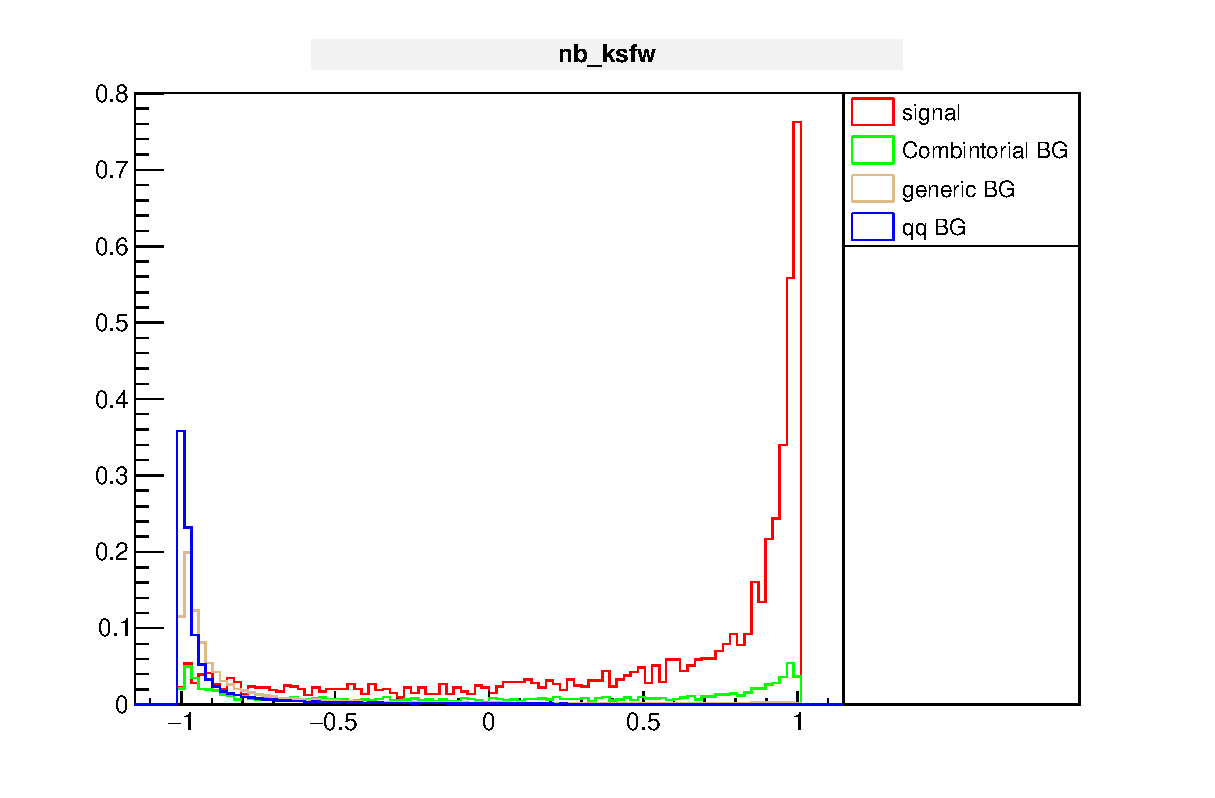
\includegraphics[width=0.45\textwidth]{bin_by_bin_study_figure/kstar1/nb_ksfw_1025_kstar1.eps}
		\label{kpi0nbksfw}
	}
	\subfigure[$K^{*\pm} \rightarrow K_s \pi^\pm$ mode.]{
		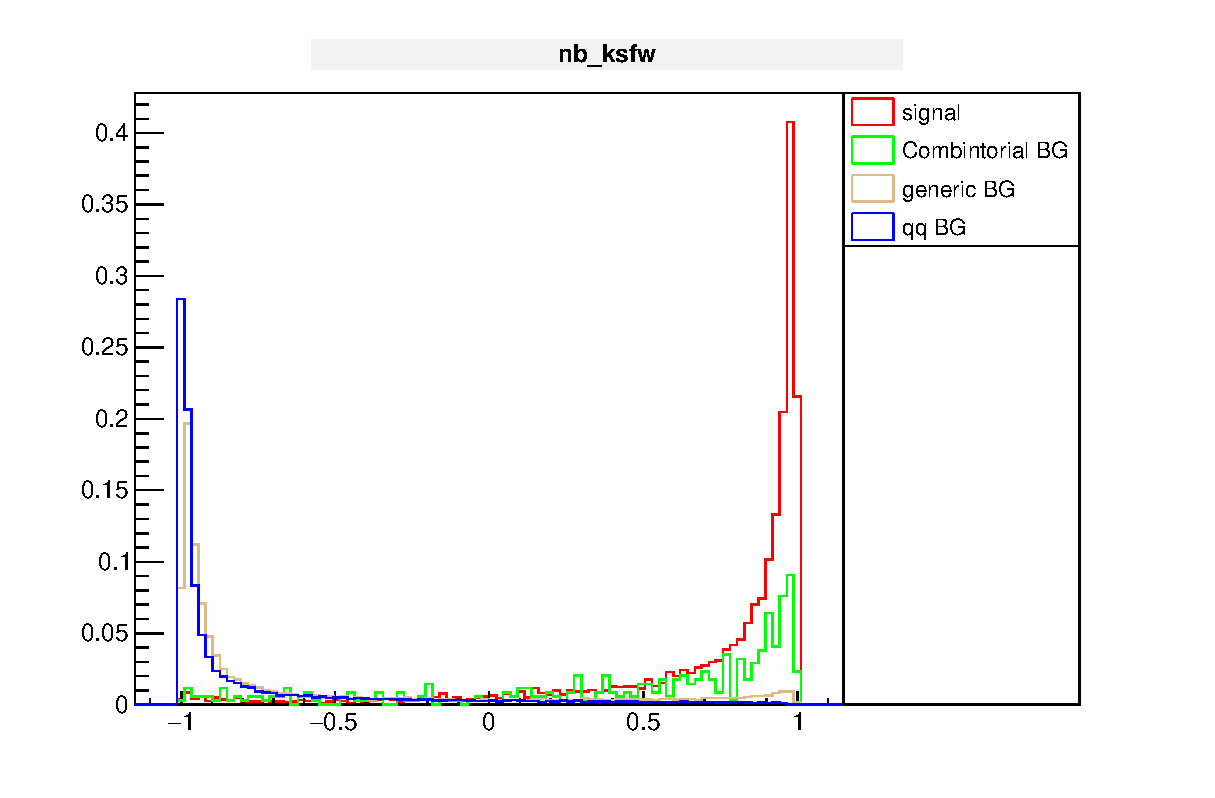
\includegraphics[width=0.45\textwidth]{bin_by_bin_study_figure/kstar2/nb_ksfw_1025_112.eps}
		\label{kspinbksfw}
	}
    \subfigure[$K^{*0}$ mode.]{
		\includegraphics[width=0.45\textwidth]{bin_by_bin_study_figure/k0/nb_ksfw_1025_1.eps}
		\label{k0nbksfw}
	}
    \subfigure[$K_s$ mode.]{
		\includegraphics[width=0.45\textwidth]{bin_by_bin_study_figure/kshort/nb_ksfw_1025_1.eps}
		\label{ksnbksfw}
	}
\caption{Neurobayes output with KSFW variables for each mode. Red line represent signal, green line represent the combinatorial background,  brown line represent the generic background and blue line represent continuum background.}
\label{fig:nbksfw}	
\end{figure}

\subsection{Optimization}
With two different variables sets of training, we get two neural-network output, there are nbvlike(variables in \ref{t:nbvlike_variables}) and nbksfw(KSFW variables). We perform the two dimensional bin-by-bin optimization on $S_b$ distribution in the signal box, which $E_{ecl} < 0.3$ by maximizing the figure of merit\cite{ref:Punzi2003}
\begin{equation}
\label{eq:fom}
\mathcal{F.O.M} = \frac{\epsilon_{sig}}{0.5 n_{\sigma}+\sqrt{N_{bkg}}},
\end{equation}
where the number of sigmas $n_\sigma$ =1.28 corresponds to one-side Gaussian limit at 90 \% CL, $\epsilon_{sig}$ is signal efficiency and $N_{bkg}$ means the expected number of background events.\\
The partial signal efficiency means the signal efficiency found within the given $S_b$ interval multiplied by the fraction of the signal efficiency distribution inside that interval.
\begin{equation}
\label{eq:peff}
\epsilon^{'sig} = \frac{N_{yield}}{N_{gen} \times R_{bin} } 
\end{equation}
The $R_{bin}$ for each bin and each mode are shown in table \ref{t:rbin} and the original $S_b$ distribution without any selection for each mode are shown in fig \ref{fig:sbcmwithotcut}. 
% \begin{table}[ht]
% \small
% \begin{center}
% \begin{tabular}{ |p{0.8cm}||p{3.7cm}||p{1.2cm}||p{1.2cm}||p{2.6cm}||p{2.7cm}| }
%  \hline
%  Bin & Partial Signal Efficiency & nbvlike & nbksfw & $N_{sig}$ & $N_{bg}$  \\
%  \hline
%  bin 1  & $(8.97 \pm 0.24) \times 10^{-4}$ &0.8&0.7&$0.657\pm 0.018 $  &$0.0\pm 1.0 $\\ % &   $1.03 \times 10^{8}$&   $2.33 \times 10^{8}$ \\
%  \hline
%  bin 2  & $(9.90 \pm 0.27)\times 10^{-4}$ &0.6& -0.2&$0.653 \pm 0.017 $&$1.0\pm 1.0 $\\ % &   $1.03 \times 10^{8}$&   $2.33 \times 10^{8}$ \\
%  \hline
%  bin 3  & $(1.37 \pm 0.03)\times 10^{-3}$ &0.5&0.6&$0.796 \pm 0.019 $&$5.40\pm 2.32 $\\ % &   $1.03 \times 10^{8}$&   $2.33 \times 10^{8}$ \\
%  \hline
%  bin 4  & $(1.63 \pm 0.04)\times 10^{-3}$ &0.4&-0.5&$0.812 \pm 0.020 $&$19.4\pm 4.41 $ \\ % &   $1.03 \times 10^{8}$&   $2.33 \times 10^{8}$ \\
%  \hline
%  bin 5  & $(1.65\pm 0.04) \times 10^{-3}$ &0.3& -0.8&$0.687 \pm 0.018 $&$33.4\pm 5.78 $ \\ % &   $1.03 \times 10^{8}$&   $2.33 \times 10^{8}$ \\
%  \hline
%  bin 6  & $(1.51\pm 0.05) \times 10^{-3}$ &0.4& -0.8&$0.50\pm 0.015 $&$35.0 \pm 5.92 $\\ % &   $1.03 \times 10^{8}$&   $2.33 \times 10^{8}$ \\
%  \hline
%  bin 7  & $(1.73 \pm 0.06)\times 10^{-3}$ &0.2&-0.8&$0.419 \pm 0.014 $&$ 54.6\pm 7.39 $ \\ % &   $1.03 \times 10^{8}$&   $2.33 \times 10^{8}$ \\
%  \hline
%  bin 8  & $(1.19 \pm 0.06)\times 10^{-3}$ &0.3&-0.8&$0.166 \pm 0.009 $&$ 40.2\pm 6.34 $ \\ % &   $1.03 \times 10^{8}$&   $2.33 \times 10^{8}$ \\
%  \hline
%  bin 9  & $(1.25 \pm 0.14)\times 10^{-3}$ &-0.3&-0.9&$0.013 \pm 0.002 $&$ 2.4\pm 1.55 $ \\ % &   $1.03 \times 10^{8}$&   $2.33 \times 10^{8}$ \\
%  \hline
%  \hline
% \end{tabular}

% \caption{Bin-by-bin optimization in signal box $E_{ecl} < 0.3$ result for $B^\pm \rightarrow K^\pm \nu \bar{\nu}$, set 0.1 for a interval on $S_b$, use 5 stream of both bb and qq MC and rare MC. Optimize with nbvlike and nbksfw 2D cut } \label{t:optk}
% \end{center}
% \end{table}

\begin{table}[h]
\small
\begin{center}
\begin{tabular}{ |p{0.8cm}||p{3.7cm}||p{1.2cm}||p{1.2cm}||p{2.6cm}||p{2.7cm}| }
 \hline
 Bin & Partial Signal Efficiency & nbvlike & nbksfw & $N_{sig}$ & $N_{bg}$  \\
 \hline
 bin 1  & $(1.65 \pm 0.03) \times 10^{-3}$ &0.2&0.7&$1.21\pm 0.024 $  &$4.22\pm 2.05 $\\ % &   $1.03 \times 10^{8}$&   $2.33 \times 10^{8}$ \\
 \hline
 bin 2  & $(1.22 \pm 0.03)\times 10^{-3}$ &0.7& 0.3&$0.807 \pm 0.019 $&$3.3\pm 1.82 $\\ % &   $1.03 \times 10^{8}$&   $2.33 \times 10^{8}$ \\
 \hline
 bin 3  & $(1.37 \pm 0.03)\times 10^{-3}$ &0.5&0.6&$0.796 \pm 0.020 $&$6.66\pm 2.58 $\\ % &   $1.03 \times 10^{8}$&   $2.33 \times 10^{8}$ \\
 \hline
 bin 4  & $(1.63 \pm 0.04)\times 10^{-3}$ &0.4&-0.5&$0.812 \pm 0.020 $&$21.0\pm 4.58 $ \\ % &   $1.03 \times 10^{8}$&   $2.33 \times 10^{8}$ \\
 \hline
 bin 5  & $(1.65\pm 0.04) \times 10^{-3}$ &0.3& -0.8&$0.687 \pm 0.018 $&$35.06\pm 5.92 $ \\ % &   $1.03 \times 10^{8}$&   $2.33 \times 10^{8}$ \\
 \hline
 bin 6  & $(1.51\pm 0.05) \times 10^{-3}$ &0.4& -0.8&$0.50\pm 0.015 $&$36.46 \pm 6.04 $\\ % &   $1.03 \times 10^{8}$&   $2.33 \times 10^{8}$ \\
 \hline
 bin 7  & $(1.73 \pm 0.06)\times 10^{-3}$ &0.2&-0.8&$0.419 \pm 0.014 $&$ 56.08\pm 7.49 $ \\ % &   $1.03 \times 10^{8}$&   $2.33 \times 10^{8}$ \\
 \hline
 bin 8  & $(1.19 \pm 0.06)\times 10^{-3}$ &0.3&-0.8&$0.166 \pm 0.009 $&$ 41.04\pm 6.41 $ \\ % &   $1.03 \times 10^{8}$&   $2.33 \times 10^{8}$ \\
 \hline
 bin 9  & $(1.25 \pm 0.14)\times 10^{-3}$ &-0.3&-0.9&$0.013 \pm 0.002 $&$ 2.44\pm 1.56 $ \\ % &   $1.03 \times 10^{8}$&   $2.33 \times 10^{8}$ \\
 \hline
 \hline
\end{tabular}

\caption{Bin-by-bin optimization in signal box $E_{ecl} < 0.3$ result for $B^\pm \rightarrow K^\pm \nu \bar{\nu}$, set 0.1 for a interval on $S_b$, use 5 stream of both bb and qq MC and rare MC. Optimize with nbvlike and nbksfw 2D cut } \label{t:optk}
\end{center}
\end{table}

\begin{table}[h]
\small
\begin{center}
\begin{tabu}to \textwidth{ |X[l]|X[c]|X[c]|X[c]|X[c]| }
\hline
 Bin & $N_{BG}$ &$N_{generic BG}$ & $N_{continuum BG}$ & $N_{rare BG}$   \\
 \hline
 bin 1  & 4.22  &0.2 &1.0&3.02\\ 
 \hline
 bin 2  & 3.3  &1.8 &0.4&1.1\\ 
 \hline
 bin 3  & 6.66  &4.6 &0.0&1.26\\ 
 \hline
 bin 4  & 21.0 	&17.8 &1.6&1.6 \\ 
 \hline
 bin 5  & 35.06  &29.2 &2.0&1.66 \\ 
 \hline
 bin 6  & 36.46 &31.6 &1.2&1.46 \\
 \hline
 bin 7  & 56.08 	&45.2 &0.6&1.48 \\ 
 \hline
  bin 8  & 41.04 	&32.2 &0.2&0.84 \\ 
 \hline
  bin 9  & 2.44 	&1.8 &0.2&0.04 \\ 
 \hline
 \hline
\end{tabu}
\caption{Background composition for $B^\pm \rightarrow K^\pm \nu \bar{\nu}$,, all the amount are scale to one data size.} \label{t:bgcomk}
\end{center}
\end{table}


\begin{figure}[ht]
\centering
\subfigure[Bin1]{
\includegraphics[width=0.2\textwidth]{bin_by_bin_study_figure/knunu/Uncert_0_1118_01bin.eps}
\label{kbin1}
}
    \subfigure[Bin2]{
\includegraphics[width=0.2\textwidth]{bin_by_bin_study_figure/knunu/Uncert_1_1118_01bin.eps}
\label{kbin2}
	}
    \subfigure[Bin3]{
\includegraphics[width=0.2\textwidth]{bin_by_bin_study_figure/knunu/Uncert_2_1118_01bin.eps}
\label{kbin3}
	}
    \subfigure[Bin4]{
\includegraphics[width=0.2\textwidth]{bin_by_bin_study_figure/knunu/Uncert_3_1118_01bin.eps}
\label{kbin4}
	}
    \subfigure[Bin5]{
\includegraphics[width=0.2\textwidth]{bin_by_bin_study_figure/knunu/Uncert_4_1118_01bin.eps}
\label{kbin5}
	}
    \subfigure[Bin6]{
\includegraphics[width=0.2\textwidth]{bin_by_bin_study_figure/knunu/Uncert_5_1118_01bin.eps}
\label{kbin6}
	}
    \subfigure[Bin7]{
\includegraphics[width=0.2\textwidth]{bin_by_bin_study_figure/knunu/Uncert_6_1118_01bin.eps}
\label{kbin7}
	}
    \subfigure[Bin8]{
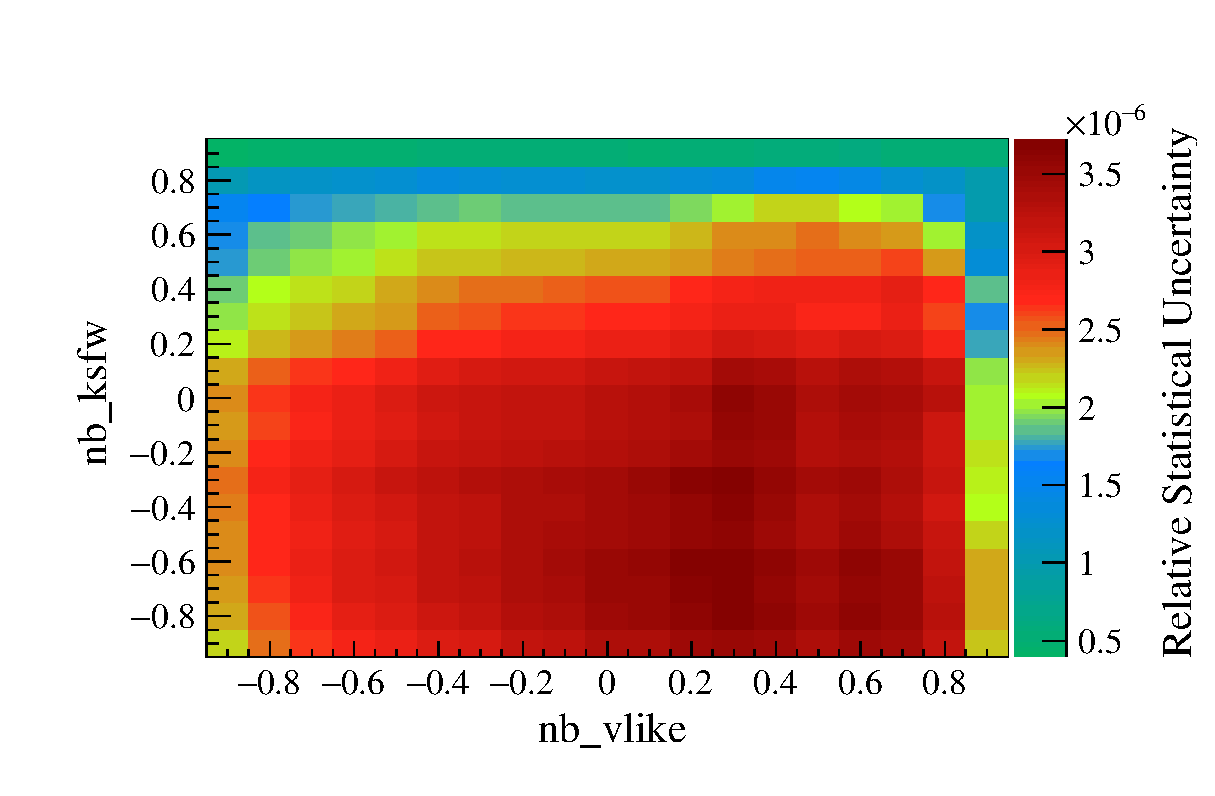
\includegraphics[width=0.2\textwidth]{bin_by_bin_study_figure/knunu/Uncert_7_1118_01bin.eps}
\label{kbin8}
	}
    \subfigure[Bin9]{
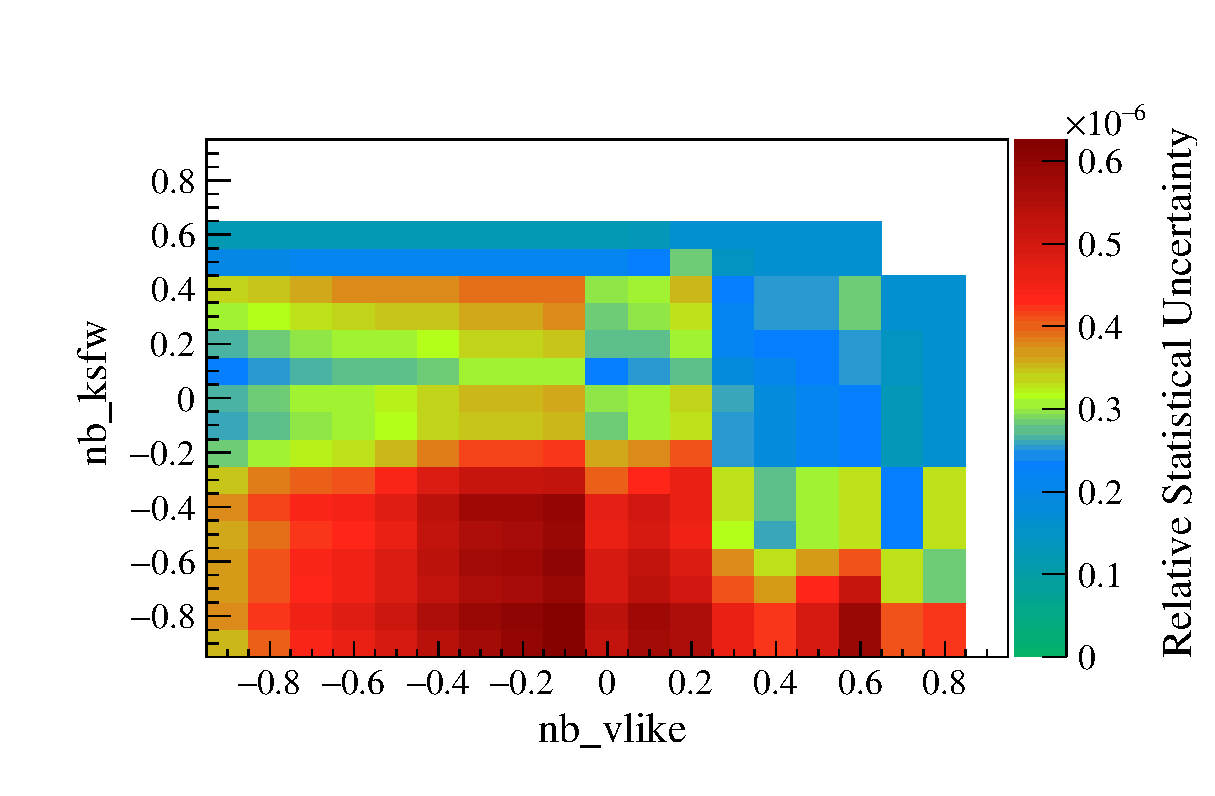
\includegraphics[width=0.2\textwidth]{bin_by_bin_study_figure/knunu/Uncert_8_1118_01bin.eps}
\label{kbin9}
	}
\caption{Two dimensional bin-by-bin $\mathcal{F.O.M.}$ plot for $B^\pm \rightarrow K^\pm \nu \bar{\nu}$.}
\label{fig:binbybinoptk}	
\end{figure}

\begin{table}[h]
\small
\begin{center}
\begin{tabular}{ |p{0.8cm}||p{3.7cm}||p{1.2cm}||p{1.2cm}||p{2.6cm}||p{2.7cm}| }
  \hline
 Bin & Partial Signal Efficiency & nbvlike & nbksfw & $N_{sig}$ & $N_{bg}$  \\
 \hline
 bin 1  & $(1.43 \pm 0.09) \times 10^{-4}$ &0.0&0.6&$0.26\pm 0.005 $  &$1.47\pm 1.21 $\\ % &   $1.03 \times 10^{8}$&   $2.33 \times 10^{8}$ \\
 \hline
 bin 2  & $(1.26 \pm 0.09)\times 10^{-4}$ &0.5& -0.9&$0.166 \pm 0.004 $&$1.57\pm 1.25 $\\ % &   $1.03 \times 10^{8}$&   $2.33 \times 10^{8}$ \\
 \hline
 bin 3  & $(1.18 \pm 0.09)\times 10^{-4}$ &0.2&0.1&$0.12 \pm 0.004 $&$1.97\pm 1.4 $\\ % &   $1.03 \times 10^{8}$&   $2.33 \times 10^{8}$ \\
 \hline
 bin 4  & $(1.20 \pm 0.10)\times 10^{-4}$ &0.1&-0.7&$0.14 \pm 0.004 $&$5.34\pm 2.31 $ \\ % &   $1.03 \times 10^{8}$&   $2.33 \times 10^{8}$ \\
 \hline
 bin 5  & $(1.11\pm 0.11) \times 10^{-4}$ &0.0& -0.9&$0.0995 \pm 0.003 $&$7.64\pm 2.76 $ \\ % &   $1.03 \times 10^{8}$&   $2.33 \times 10^{8}$ \\
 \hline
 bin 6  & $(1.18\pm 0.14) \times 10^{-4}$ &-0.6& -0.9&$0.078\pm 0.003 $&$21.97 \pm 4.69 $\\ % &   $1.03 \times 10^{8}$&   $2.33 \times 10^{8}$ \\
 \hline
 bin 7  & $(3.73 \pm 1.14)\times 10^{-5}$ &-0.1&0.2&$0.0109 \pm 0.001 $&$ 2.4\pm 1.55 $ \\ % &   $1.03 \times 10^{8}$&   $2.33 \times 10^{8}$ \\
 \hline
 \hline
\end{tabular}

\caption{Bin-by-bin optimization in signal box $E_{ecl} < 0.3$ result for $K^{*\pm} \rightarrow K^{+} \pi^0$, set 0.1 for a interval on $S_b$, use 5 stream of both bb and qq MC and rare MC. Optimize with nbvlike and nbksfw 2D cut } \label{t:optkpi0}
\end{center}
\end{table}

\begin{table}[h]
\small
\begin{center}
\begin{tabu}to \textwidth{ |X[l]|X[c]|X[c]|X[c]|X[c]| }
\hline
 Bin & $N_{BG}$ &$N_{generic BG}$ & $N_{continuum BG}$ & $N_{rare BG}$   \\
 \hline
 bin 1  & 1.47  &0 &0.2&1.26\\ 
 \hline
 bin 2  & 1.57  &1.0 &0.2&0.36\\ 
 \hline
 bin 3  & 1.97  &1.0 &0.4&0.56\\ 
 \hline
 bin 4  & 5.34 	&4.4 &0.4&0.52 \\ 
 \hline
 bin 5  & 7.64  &7 &0.2&0.42 \\ 
 \hline
 bin 6  & 21.97 &19.2 &2.2&0.54 \\
 \hline
 bin 7  & 2.4 	&2.2 &0.2&0.04 \\ 
 \hline
 \hline
\end{tabu}
\caption{Background composition for $K^* \rightarrow K \pi^0$, all the amount are scale to one data size.} \label{t:bgcomkpi0}
\end{center}
\end{table}




% \begin{table}[h]
% \small
% \begin{center}
% \begin{tabular}{ |p{0.8cm}||p{3.7cm}||p{1.2cm}||p{1.2cm}||p{2.6cm}||p{2.7cm}| }
%   \hline
%  Bin & Partial Signal Efficiency & nbvlike & nbksfw & $N_{sig}$ & $N_{bg}$  \\
%  \hline
%  bin 1  & $(1.43 \pm 0.09) \times 10^{-4}$ &0.0&0.6&$0.26\pm 0.005 $  &$0.21\pm 0.458 $\\ % &   $1.03 \times 10^{8}$&   $2.33 \times 10^{8}$ \\
%  \hline
%  bin 2  & $(1.03 \pm 0.08)\times 10^{-4}$ &0.6& 0.5&$0.166 \pm 0.004 $&$0.606\pm 0.778 $\\ % &   $1.03 \times 10^{8}$&   $2.33 \times 10^{8}$ \\
%  \hline
%  bin 3  & $(8.59 \pm 0.80)\times 10^{-5}$ &0.2&0.8&$0.12 \pm 0.004 $&$0.41\pm 0.64 $\\ % &   $1.03 \times 10^{8}$&   $2.33 \times 10^{8}$ \\
%  \hline
%  bin 4  & $(1.20 \pm 0.10)\times 10^{-4}$ &0.1&-0.7&$0.14 \pm 0.004 $&$4.8\pm 2.19 $ \\ % &   $1.03 \times 10^{8}$&   $2.33 \times 10^{8}$ \\
%  \hline
%  bin 5  & $(1.07\pm 0.11) \times 10^{-4}$ &0.0& -0.9&$0.0995 \pm 0.003 $&$7.22\pm 2.69 $ \\ % &   $1.03 \times 10^{8}$&   $2.33 \times 10^{8}$ \\
%  \hline
%  bin 6  & $(1.18\pm 0.14) \times 10^{-4}$ &-0.6& -0.9&$0.078\pm 0.003 $&$21.43 \pm 4.63 $\\ % &   $1.03 \times 10^{8}$&   $2.33 \times 10^{8}$ \\
%  \hline
%  bin 7  & $(3.73 \pm 1.10)\times 10^{-5}$ &-0.1&0.2&$0.0109 \pm 0.001 $&$ 2.4\pm 1.55 $ \\ % &   $1.03 \times 10^{8}$&   $2.33 \times 10^{8}$ \\
%  \hline
%  \hline
% \end{tabular}

% \caption{Bin-by-bin optimization in signal box $E_{ecl} < 0.3$ result for $K^{*\pm} \rightarrow K^{+} \pi^0$, set 0.1 for a interval on $S_b$, use 5 stream of both bb and qq MC. Optimize with nbvlike and nbksfw 2D cut } \label{t:optkpi0}
% \end{center}
% \end{table}

\begin{figure}[ht]
\centering
\subfigure[Bin1]{
\includegraphics[width=0.2\textwidth]{bin_by_bin_study_figure/kstar1/Uncert_0_1118_01bin.eps}
\label{kpi0bin1}
}
    \subfigure[Bin2]{
\includegraphics[width=0.2\textwidth]{bin_by_bin_study_figure/kstar1/Uncert_1_1118_01bin.eps}
\label{kpi0bin2}
	}
    \subfigure[Bin3]{
\includegraphics[width=0.2\textwidth]{bin_by_bin_study_figure/kstar1/Uncert_2_1118_01bin.eps}
\label{kpi0bin3}
	}
    \subfigure[Bin4]{
\includegraphics[width=0.2\textwidth]{bin_by_bin_study_figure/kstar1/Uncert_3_1118_01bin.eps}
\label{kpi0bin4}
	}
    \subfigure[Bin5]{
\includegraphics[width=0.2\textwidth]{bin_by_bin_study_figure/kstar1/Uncert_4_1118_01bin.eps}
\label{kpi0bin5}
	}
    \subfigure[Bin6]{
\includegraphics[width=0.2\textwidth]{bin_by_bin_study_figure/kstar1/Uncert_5_1118_01bin.eps}
\label{kpi0bin6}
	}
    \subfigure[Bin7]{
\includegraphics[width=0.2\textwidth]{bin_by_bin_study_figure/kstar1/Uncert_6_1118_01bin.eps}
\label{kpi0bin7}
	}
\caption{Two dimensional bin-by-bin $\mathcal{F.O.M.}$ plot for $K^{*\pm} \rightarrow K^{+} \pi^0$ .}
\label{fig:binbybinoptkpi0}	
\end{figure}

% \begin{table}[ht]
% \small
% \begin{center}
% \begin{tabular}{ |p{0.8cm}||p{3.7cm}||p{1.2cm}||p{1.2cm}||p{2.6cm}||p{2.7cm}| }
%  \hline
%  Bin & Signal Efficiency & nbvlike & nbksfw & $N_{sig}$ & $N_{bg}$  \\
%  \hline
%  bin 1  & $(1.32 \pm 0.086) \times 10^{-4}$ &0.9&0.7&$0.24\pm 0.004 $  &$0.0002\pm 0.016 $\\ % &   $1.03 \times 10^{8}$&   $2.33 \times 10^{8}$ \\
%  \hline
%  bin 2  & $(2.21 \pm 0.012)\times 10^{-4}$ &0.3& 0.6&$0.357 \pm 0.004 $&$1.80\pm 1.34 $\\ % &   $1.03 \times 10^{8}$&   $2.33 \times 10^{8}$ \\
%  \hline
%  bin 3  & $(1.96 \pm 0.012)\times 10^{-4}$ &0.7&-0.5&$0.274 \pm 0.003 $&$1.60\pm 1.26 $\\ % &   $1.03 \times 10^{8}$&   $2.33 \times 10^{8}$ \\
%  \hline
%  bin 4  & $(1.78 \pm 0.012)\times 10^{-4}$ &0.5&-0.1&$0.208 \pm 0.003 $&$3.80\pm 1.95 $ \\ % &   $1.03 \times 10^{8}$&   $2.33 \times 10^{8}$ \\
%  \hline
%  bin 5  & $(1.28\pm 0.12) \times 10^{-4}$ &0.8& -0.5&$0.119 \pm 0.003 $&$3.20\pm 1.79 $ \\ % &   $1.03 \times 10^{8}$&   $2.33 \times 10^{8}$ \\
%  \hline
%  bin 6  & $(1.11\pm 0.13) \times 10^{-4}$ &0.8& 0.1&$0.073\pm 0.002 $&$2.40 \pm 1.55 $\\ % &   $1.03 \times 10^{8}$&   $2.33 \times 10^{8}$ \\
%  \hline
%  bin 7  & $(6.3 \pm 1.0)\times 10^{-5}$ &0.7&-0.9&$0.035 \pm 0.001 $&$ 2.60\pm 1.61 $ \\ % &   $1.03 \times 10^{8}$&   $2.33 \times 10^{8}$ \\
%  \hline
%  \hline
% \end{tabular}

% \caption{Bin-by-bin optimization in signal box $E_{ecl} < 0.3$ result for $K^* \rightarrow K_s \pi^+$, set 0.1 for a interval on $S_b$, use 5 stream of both bb and qq MC. Optimize with nbvlike and nbksfw 2D cut } \label{t:optkspi}
% \end{center}
% \end{table}
\clearpage

\begin{table}[h]
\small
\begin{center}
\begin{tabular}{ |p{0.8cm}||p{3.7cm}||p{1.2cm}||p{1.2cm}||p{2.6cm}||p{2.7cm}| }
 \hline
 Bin & Signal Efficiency & nbvlike & nbksfw & $N_{sig}$ & $N_{bg}$  \\
 \hline
 bin 1  & $(2.54 \pm 0.12) \times 10^{-4}$ &0.4&0.6&$0.46\pm 0.005 $  &$2.34\pm 1.53 $\\ % &   $1.03 \times 10^{8}$&   $2.33 \times 10^{8}$ \\
 \hline
 bin 2  & $(2.38 \pm 0.12)\times 10^{-4}$ &0.2& 0.8&$0.385 \pm 0.004 $&$2.54\pm 1.59 $\\ % &   $1.03 \times 10^{8}$&   $2.33 \times 10^{8}$ \\
 \hline
 bin 3  & $(2.41 \pm 0.13)\times 10^{-4}$ &0.6&-0.1&$0.337 \pm 0.003 $&$2.98\pm 1.73 $\\ % &   $1.03 \times 10^{8}$&   $2.33 \times 10^{8}$ \\
 \hline
 bin 4  & $(1.99 \pm 0.13)\times 10^{-4}$ &0.6&0.0&$0.233 \pm 0.002 $&$4.48\pm 2.11 $ \\ % &   $1.03 \times 10^{8}$&   $2.33 \times 10^{8}$ \\
 \hline
 bin 5  & $(1.58\pm 0.13) \times 10^{-4}$ &0.8& -0.5&$0.147 \pm 0.001 $&$4.66\pm 2.16 $ \\ % &   $1.03 \times 10^{8}$&   $2.33 \times 10^{8}$ \\
 \hline
 bin 6  & $(1.34\pm 0.14) \times 10^{-4}$ &0.8& -0.1&$0.088\pm 0.001 $&$4.24 \pm 2.06 $\\ % &   $1.03 \times 10^{8}$&   $2.33 \times 10^{8}$ \\
 \hline
 bin 7  & $(8.35 \pm 1.24)\times 10^{-5}$ &0.4&-0.6&$0.046 \pm 0.0004 $&$ 4.08\pm 2.02 $ \\ % &   $1.03 \times 10^{8}$&   $2.33 \times 10^{8}$ \\
 \hline
 \hline
\end{tabular}

\caption{Bin-by-bin optimization in signal box $E_{ecl} < 0.3$ result for $K^* \rightarrow K_s \pi^+$, set 0.1 for a interval on $S_b$, use 5 stream of both bb and qq MC and rare MC. Optimize with nbvlike and nbksfw 2D cut } \label{t:optkspi}
\end{center}
\end{table}

\begin{table}[h]
\small
\begin{center}
\begin{tabu}to \textwidth{ |X[l]|X[c]|X[c]|X[c]|X[c]| }
\hline
 Bin & $N_{BG}$ &$N_{generic BG}$ & $N_{continuum BG}$ & $N_{rare BG}$   \\
 \hline
 bin 1  & 2.34  &0.2 &1.0&1.14\\ 
 \hline
 bin 2  & 2.54  &1.4 &0.4&0.74\\ 
 \hline
 bin 3  & 2.98  &1.6 &0.8&0.58\\ 
 \hline
 bin 4  & 4.48 	&3.2 &0.8&0.48 \\ 
 \hline
 bin 5  & 4.66  &3.8 &0.6&0.26 \\ 
 \hline
 bin 6  & 4.24 	&3.4 &0.6&0.24 \\
 \hline
 bin 7  & 4.08 	&3.4 &0.6&0.08 \\ 
 \hline
 \hline
\end{tabu}
\caption{Background composition for $K^* \rightarrow K_s \pi^+$, all the amount are scale to one data size.} \label{t:bgcomkspi}
\end{center}
\end{table}






\begin{figure}[ht]
\centering
\subfigure[Bin1]{
\includegraphics[width=0.2\textwidth]{bin_by_bin_study_figure/kstar2/Uncert_0_1118_01bin11.eps}
\label{kspibin1}
}
\subfigure[Bin2]{
\includegraphics[width=0.2\textwidth]{bin_by_bin_study_figure/kstar2/Uncert_1_1118_01bin11.eps}
\label{kspibin2}
}
\subfigure[Bin3]{
\includegraphics[width=0.2\textwidth]{bin_by_bin_study_figure/kstar2/Uncert_2_1118_01bin11.eps}
\label{kspibin3}
}
\subfigure[Bin4]{
\includegraphics[width=0.2\textwidth]{bin_by_bin_study_figure/kstar2/Uncert_3_1118_01bin11.eps}
\label{kspibin4}
}
\subfigure[Bin5]{
\includegraphics[width=0.2\textwidth]{bin_by_bin_study_figure/kstar2/Uncert_4_1118_01bin11.eps}
\label{kspibin5}
}
\subfigure[Bin6]{
\includegraphics[width=0.2\textwidth]{bin_by_bin_study_figure/kstar2/Uncert_5_1118_01bin11.eps}
\label{kspibin6}
}
\subfigure[Bin7]{
\includegraphics[width=0.2\textwidth]{bin_by_bin_study_figure/kstar2/Uncert_6_1118_01bin11.eps}
\label{kspibin7}
}
\caption{Two dimensional bin-by-bin $\mathcal{F.O.M.}$ plot for $K^{*\pm} \rightarrow K_s \pi^+$ .}
\label{fig:binbybinoptkspi}	
\end{figure}

\begin{table}[h]
\small
\begin{center}
\begin{tabular}{ |p{0.8cm}||p{3.7cm}||p{1.2cm}||p{1.2cm}||p{2.6cm}||p{2.7cm}| }
\hline
 Bin & Signal Efficiency & nbvlike & nbksfw & $N_{sig}$ & $N_{bg}$  \\
 \hline
 bin 1  & $(6.01 \pm 0.183) \times 10^{-4}$ &-0.2&0.5&$1.02\pm 0.015 $  &$9.84\pm 3.14 $\\ % &   $1.03 \times 10^{8}$&   $2.33 \times 10^{8}$ \\
 \hline
 bin 2  & $(5.22 \pm 0.182)\times 10^{-4}$ &0.2& 0.0&$0.784 \pm 0.012 $&$6.0\pm 2.45 $\\ % &   $1.03 \times 10^{8}$&   $2.33 \times 10^{8}$ \\
 \hline
 bin 3  & $(4.03 \pm 0.172)\times 10^{-4}$ &0.7&-0.3&$0.522 \pm 0.009 $&$3.64\pm 1.91 $\\ % &   $1.03 \times 10^{8}$&   $2.33 \times 10^{8}$ \\
 \hline
 bin 4  & $(4.82 \pm 0.206)\times 10^{-4}$ &0.2&0.0&$0.522 \pm 0.009 $&$16.28\pm 4.03 $ \\ % &   $1.03 \times 10^{8}$&   $2.33 \times 10^{8}$ \\
 \hline
 bin 5  & $(3.08\pm 0.184) \times 10^{-4}$ &0.8& 0.2&$0.264 \pm 0.002 $&$5.0\pm 2.24 $ \\ % &   $1.03 \times 10^{8}$&   $2.33 \times 10^{8}$ \\
 \hline
 bin 6  & $(4.44\pm 0.26) \times 10^{-4}$ &0.3& -0.6&$0.269\pm 0.005 $&$24.34 \pm 4.93 $\\ % &   $1.03 \times 10^{8}$&   $2.33 \times 10^{8}$ \\
 \hline
 bin 7  & $(3.03 \pm 0.33)\times 10^{-4}$ &0.3&-0.6&$0.081 \pm 0.002 $&$ 14.52\pm 3.81 $ \\ % &   $1.03 \times 10^{8}$&   $2.33 \times 10^{8}$ \\
 \hline
 \hline
\end{tabular}

\caption{Bin-by-bin optimization in signal box $E_{ecl} < 0.3$ result for $B^0 \rightarrow K^{(*0)} \nu \bar{\nu}$, set 0.1 for a interval on $S_b$, use 5 stream of both bb and qq MC and rare MC. Optimize with nbvlike and nbksfw 2D cut } \label{t:optk0}
\end{center}
\end{table}

\begin{table}[h]
\small
\begin{center}
\begin{tabu}to \textwidth{ |X[l]|X[c]|X[c]|X[c]|X[c]| }
\hline
 Bin & $N_{BG}$ &$N_{generic BG}$ & $N_{continuum BG}$ & $N_{rare BG}$   \\
 \hline
 bin 1  & 9.84  &0.8 &3.4&5.64\\ 
 \hline
 bin 2  & 6.0  	&2.4 &1.0&2.6\\ 
 \hline
 bin 3  & 3.64  &2.0 &0.0&1.64\\ 
 \hline
 bin 4  & 16.28 &13.2&1.2&1.88 \\ 
 \hline
 bin 5  & 5.0   &4.2 &0.2&0.6 \\ 
 \hline
 bin 6  & 24.84 &19.2&4.2&1.44 \\
 \hline
 bin 7  & 14.52 &12.4&1.6&0.52 \\ 
 \hline
 \hline
\end{tabu}
\caption{Background composition for $B^0 \rightarrow K^0 \nu \bar{\nu}$, all the amount are scale to one data size.} \label{t:bgcomk0}
\end{center}
\end{table}

% \begin{table}[ht]
% \small
% \begin{center}
% \begin{tabular}{ |p{0.8cm}||p{3.7cm}||p{1.2cm}||p{1.2cm}||p{2.6cm}||p{2.7cm}| }
% \hline
%  Bin & Signal Efficiency & nbvlike & nbksfw & $N_{sig}$ & $N_{bg}$  \\
%  \hline
%  bin 1  & $(2.22 \pm 0.113) \times 10^{-4}$ &0.9&-0.9&$0.377\pm 0.009 $  &$0.0\pm 1.0 $\\ % &   $1.03 \times 10^{8}$&   $2.33 \times 10^{8}$ \\
%  \hline
%  bin 2  & $(5.1 \pm 0.179)\times 10^{-4}$ &0.3& -0.2&$0.76 \pm 0.012 $&$3.0\pm 1.73 $\\ % &   $1.03 \times 10^{8}$&   $2.33 \times 10^{8}$ \\
%  \hline
%  bin 3  & $(3.36 \pm 0.157)\times 10^{-4}$ &0.8&0.3&$0.435 \pm 0.009 $&$1.0\pm 1.0 $\\ % &   $1.03 \times 10^{8}$&   $2.33 \times 10^{8}$ \\
%  \hline
%  bin 4  & $(4.82 \pm 0.206)\times 10^{-4}$ &0.2&0.0&$0.522 \pm 0.009 $&$14.4\pm 3.79 $ \\ % &   $1.03 \times 10^{8}$&   $2.33 \times 10^{8}$ \\
%  \hline
%  bin 5  & $(3.08\pm 0.184) \times 10^{-4}$ &0.8& 0.2&$0.264 \pm 0.002 $&$4.4\pm 2.10 $ \\ % &   $1.03 \times 10^{8}$&   $2.33 \times 10^{8}$ \\
%  \hline
%  bin 6  & $(4.44\pm 0.26) \times 10^{-4}$ &0.3& -0.6&$0.269\pm 0.005 $&$23.4 \pm 4.84 $\\ % &   $1.03 \times 10^{8}$&   $2.33 \times 10^{8}$ \\
%  \hline
%  bin 7  & $(3.03 \pm 0.33)\times 10^{-4}$ &0.3&-0.6&$0.081 \pm 0.002 $&$ 14.0\pm 3.74 $ \\ % &   $1.03 \times 10^{8}$&   $2.33 \times 10^{8}$ \\
%  \hline
%  \hline
% \end{tabular}

% \caption{Bin-by-bin optimization in signal box $E_{ecl} < 0.3$ result for $B^0 \rightarrow K^{(*0)} \nu \bar{\nu}$, set 0.1 for a interval on $S_b$, use 5 stream of both bb and qq MC. Optimize with nbvlike and nbksfw 2D cut } \label{t:optkspi}
% \end{center}
% \end{table}

\begin{figure}[ht]
\centering
\subfigure[Bin1]{
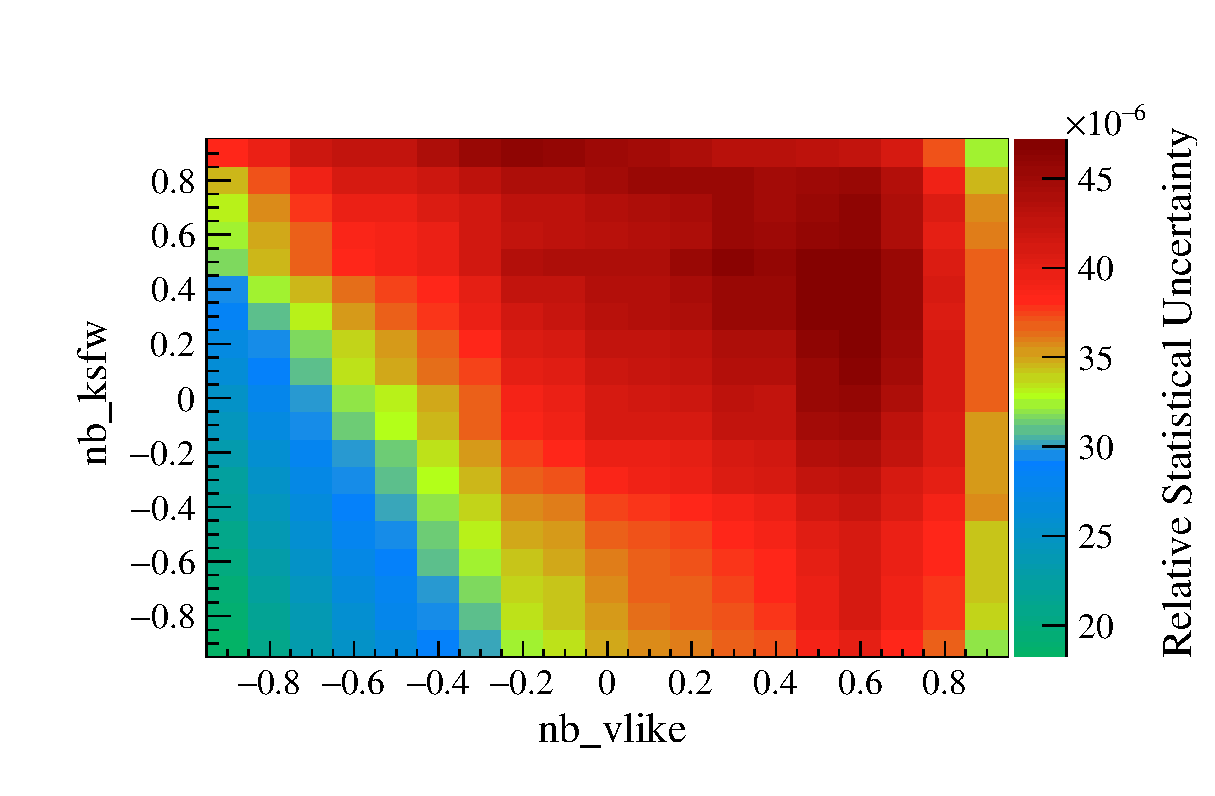
\includegraphics[width=0.2\textwidth]{bin_by_bin_study_figure/k0/Uncert_0_1115_01bin.eps}
\label{k0bin1}
}
\subfigure[Bin2]{
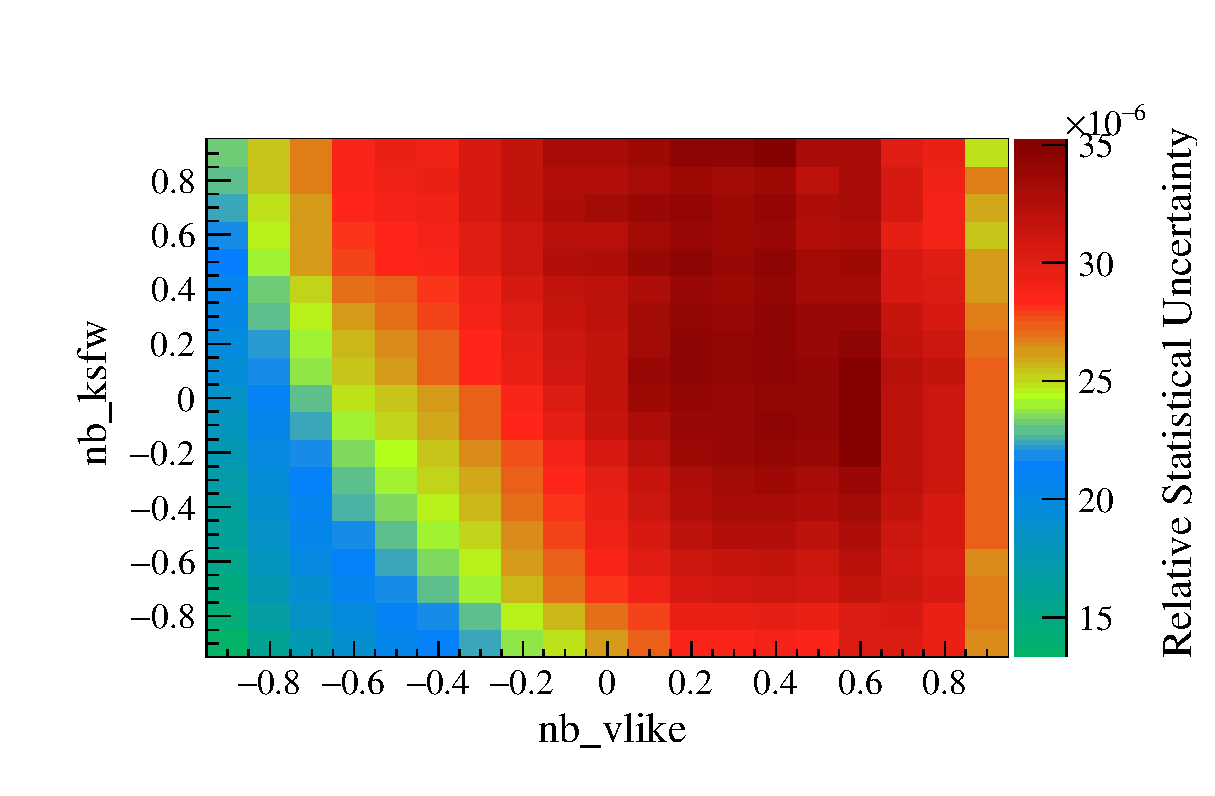
\includegraphics[width=0.2\textwidth]{bin_by_bin_study_figure/k0/Uncert_1_1115_01bin.eps}
\label{k0bin1}
}
\subfigure[Bin3]{
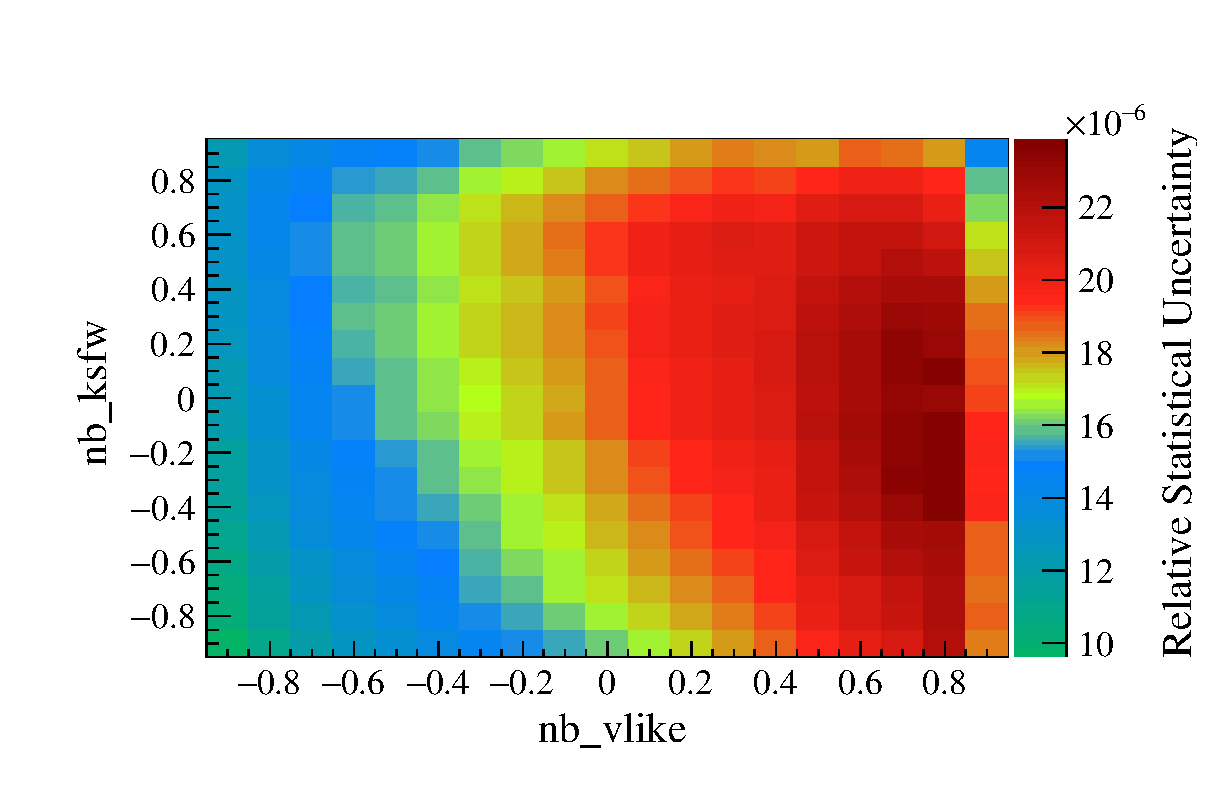
\includegraphics[width=0.2\textwidth]{bin_by_bin_study_figure/k0/Uncert_2_1115_01bin.eps}
\label{k0bin1}
}
\subfigure[Bin4]{
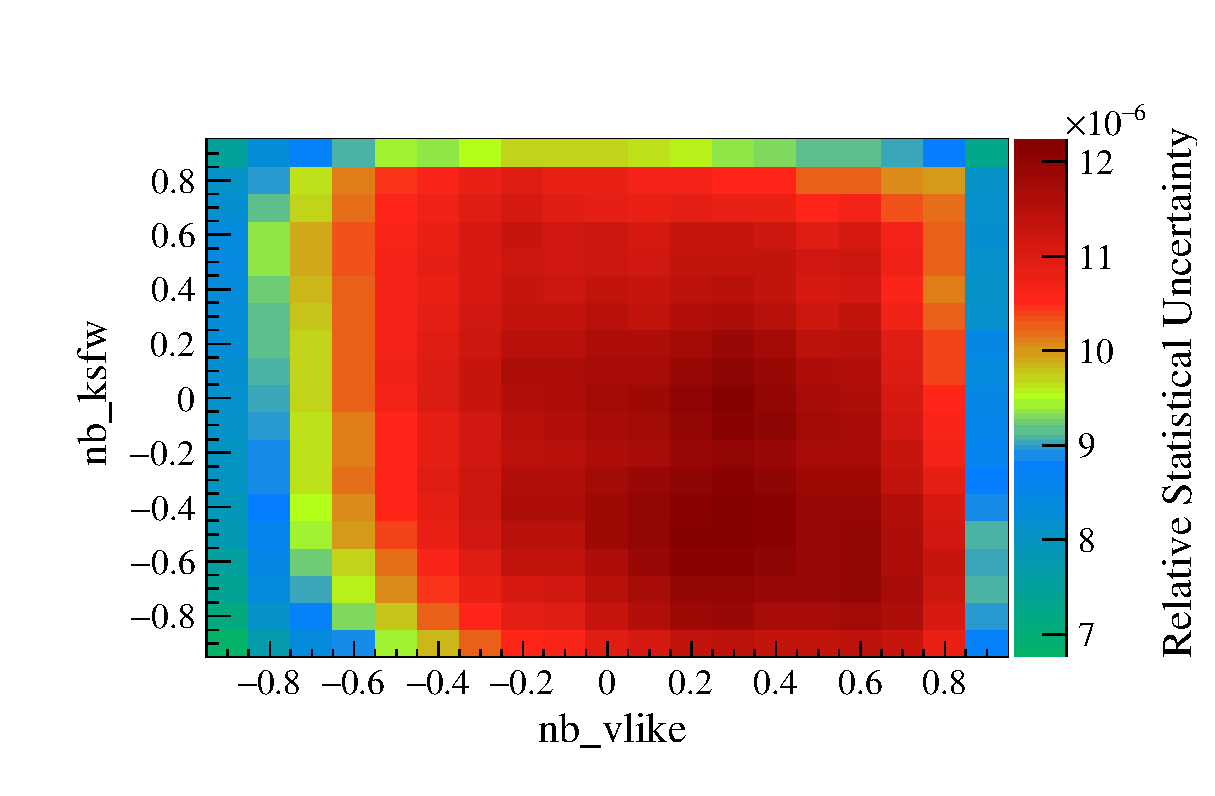
\includegraphics[width=0.2\textwidth]{bin_by_bin_study_figure/k0/Uncert_3_1115_01bin.eps}
\label{k0bin1}
}
\subfigure[Bin5]{
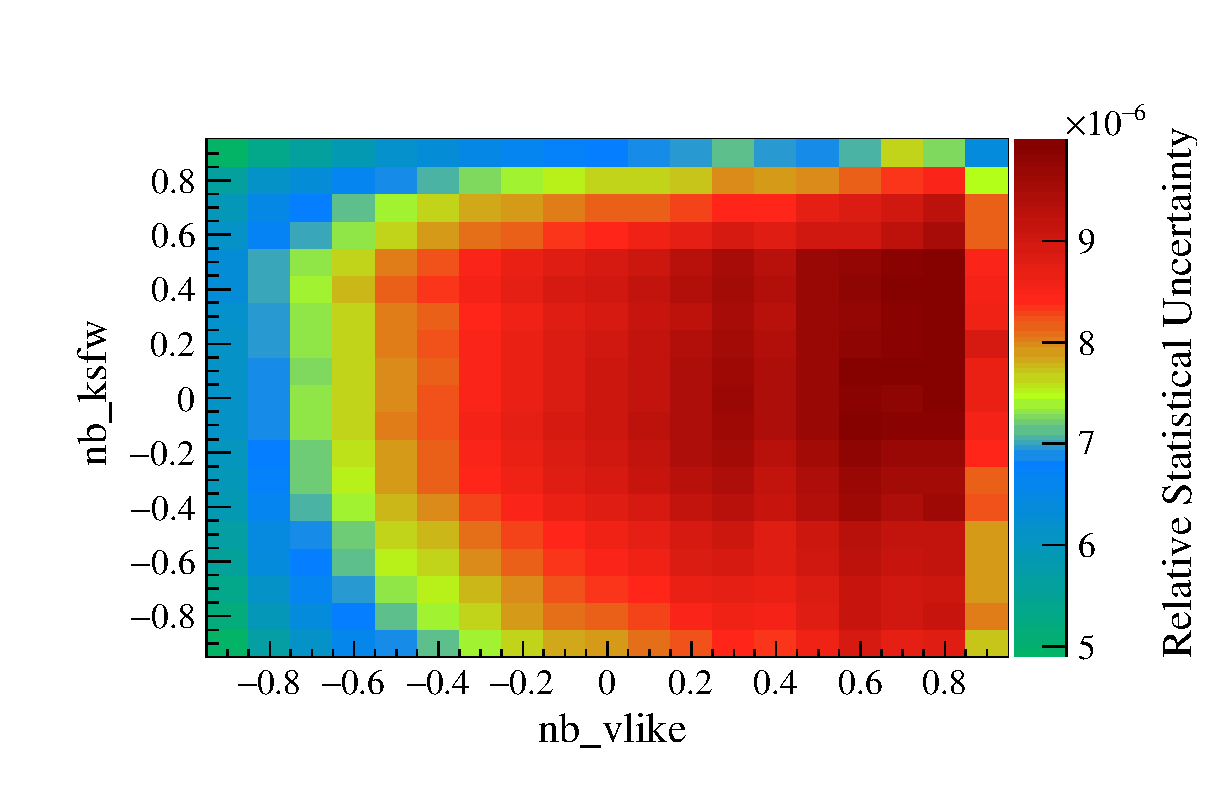
\includegraphics[width=0.2\textwidth]{bin_by_bin_study_figure/k0/Uncert_4_1115_01bin.eps}
\label{k0bin1}
}
\subfigure[Bin6]{
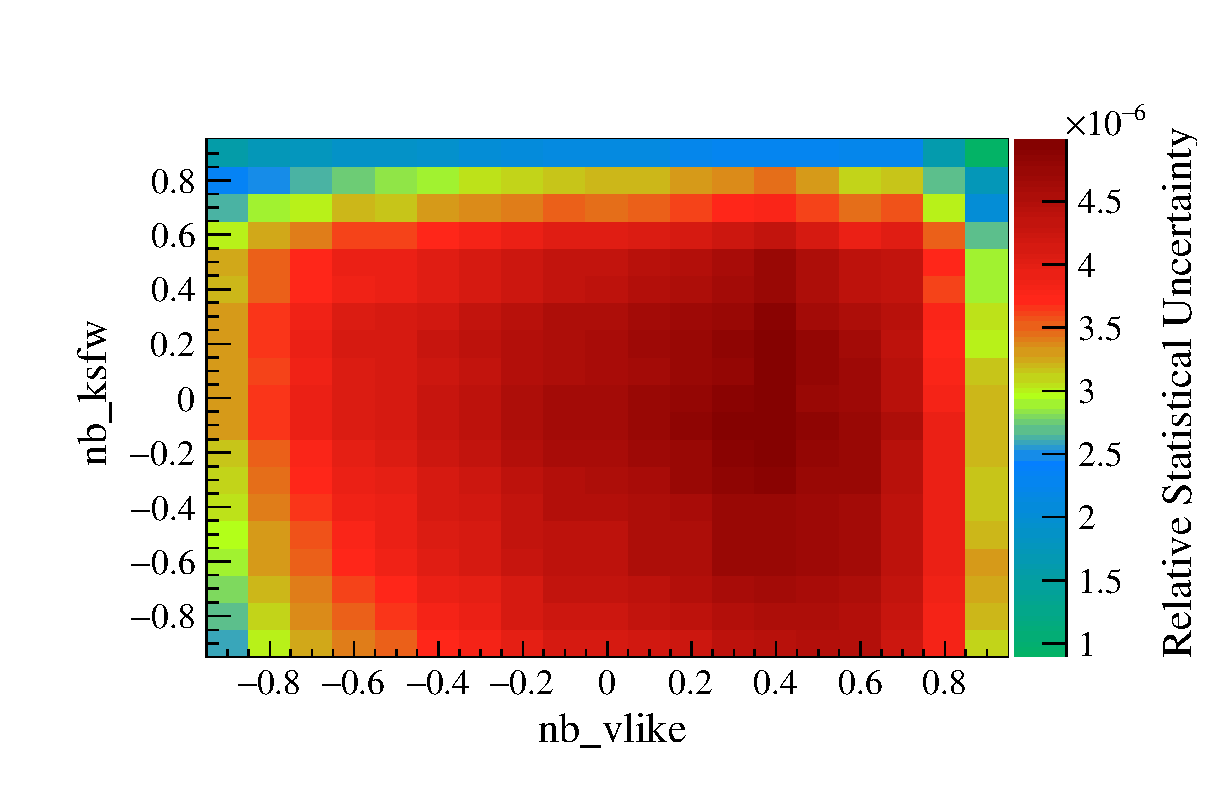
\includegraphics[width=0.2\textwidth]{bin_by_bin_study_figure/k0/Uncert_5_1115_01bin.eps}
\label{k0bin1}
}
\subfigure[Bin7]{
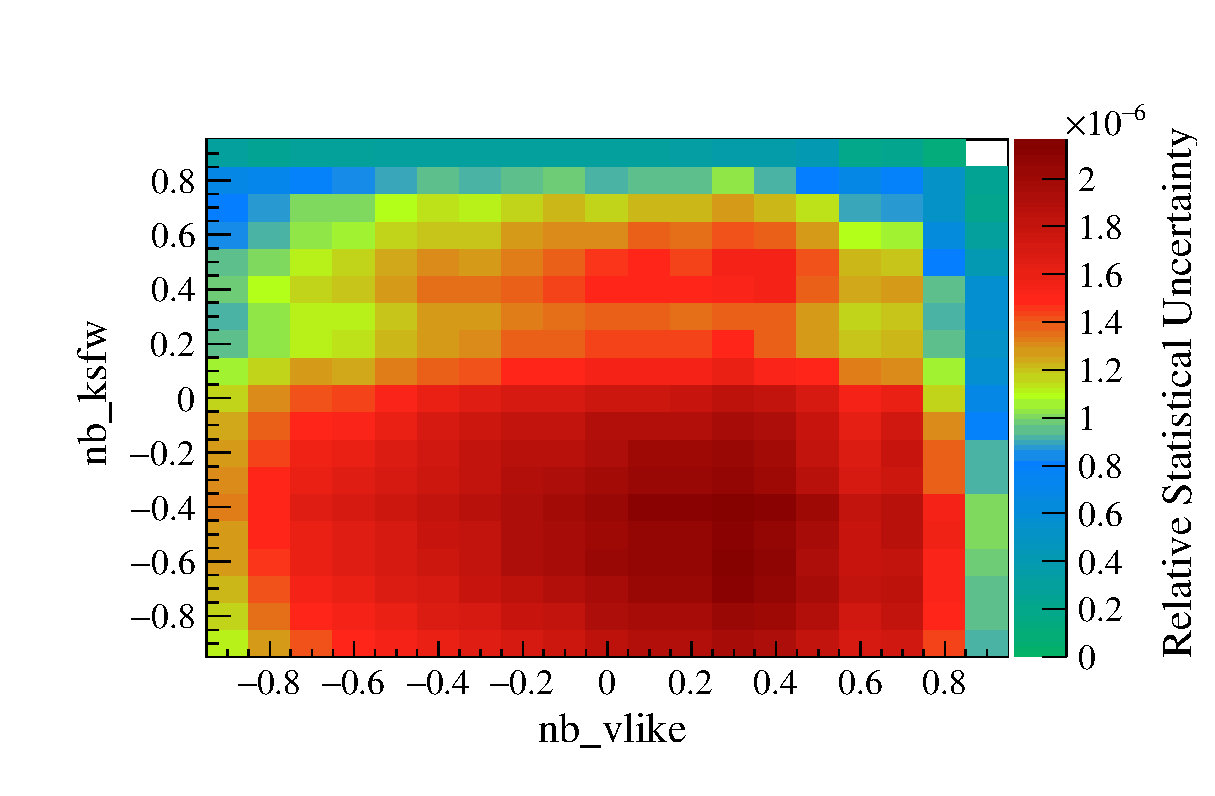
\includegraphics[width=0.2\textwidth]{bin_by_bin_study_figure/k0/Uncert_6_1115_01bin.eps}
\label{k0bin1}
}
\caption{Two dimensional bin-by-bin $\mathcal{F.O.M.}$ plot for $B^0 \rightarrow K^{(*0)} \nu \bar{\nu}$.}
\label{fig:binbybinoptkspi}	
\end{figure}


% \begin{table}[ht]
% \small
% \begin{center}
% \begin{tabular}{ |p{0.8cm}||p{3.7cm}||p{1.2cm}||p{1.2cm}||p{2.6cm}||p{2.7cm}| }
% \hline
%  Bin & Signal Efficiency & nbvlike & nbksfw & $N_{sig}$ & $N_{bg}$  \\
%  \hline
%  bin 1  & $(8.74 \pm 0.23) \times 10^{-4}$ &0.6&0.6&$0.301\pm 0.008 $  &$0.2\pm 0.447 $\\ % &   $1.03 \times 10^{8}$&   $2.33 \times 10^{8}$ \\
%  \hline
%  bin 2  & $(6.9 \pm 0.22)\times 10^{-4}$ &0.6& 0.9&$0.211 \pm 0.007 $&$0.2\pm 0.447 $\\ % &   $1.03 \times 10^{8}$&   $2.33 \times 10^{8}$ \\
%  \hline
%  bin 3  & $(9.97 \pm 0.28)\times 10^{-4}$ &0.5&-0.91&$0.267 \pm 0.008 $&$1.8\pm 1.34 $\\ % &   $1.03 \times 10^{8}$&   $2.33 \times 10^{8}$ \\
%  \hline
%  bin 4  & $(7.76\pm 0.27)\times 10^{-4}$ &0.6&0.2&$0.179 \pm 0.006 $&$4.2\pm 2.05 $ \\ % &   $1.03 \times 10^{8}$&   $2.33 \times 10^{8}$ \\
%  \hline
%  bin 5  & $(6.81\pm 0.28) \times 10^{-4}$ &0.7& 0.5&$0.131 \pm 0.005 $&$3.8\pm 1.95 $ \\ % &   $1.03 \times 10^{8}$&   $2.33 \times 10^{8}$ \\
%  \hline
%  bin 6  & $(6.52\pm 0.304) \times 10^{-4}$ &0.7& -0.9&$0.0998\pm 0.005 $&$5.8 \pm 2.41 $\\ % &   $1.03 \times 10^{8}$&   $2.33 \times 10^{8}$ \\
%  \hline
%  bin 7  & $(6.77 \pm 0.36)\times 10^{-4}$ &0.2&-0.4&$0.0754 \pm 0.004 $&$ 12.6\pm 3.55 $ \\ % &   $1.03 \times 10^{8}$&   $2.33 \times 10^{8}$ \\
% \hline
%  bin 8  & $(1.62 \pm 0.46)\times 10^{-4}$ &0.6&0.0&$0.0839 \pm 0.0043 $&$ 32.600\pm 5.710 $ \\ % &   $1.03 \times 10^{8}$&   $2.33 \times 10^{8}$ \\
%  \hline
%  \hline
% \end{tabular}
\begin{table}[h]
\small
\begin{center}
\begin{tabular}{ |p{0.8cm}||p{3.7cm}||p{1.2cm}||p{1.2cm}||p{2.6cm}||p{2.7cm}| }
\hline
 Bin & Signal Efficiency & nbvlike & nbksfw & $N_{sig}$ & $N_{bg}$  \\
 \hline
 bin 1  & $(9.57 \pm 0.25) \times 10^{-4}$ &0.3&0.6&$0.329\pm 0.008 $  &$1.24\pm 1.11 $\\ % &   $1.03 \times 10^{8}$&   $2.33 \times 10^{8}$ \\
 \hline
 bin 2  & $(6.9 \pm 0.22)\times 10^{-4}$ &0.6& 0.9&$0.211 \pm 0.007 $&$0.66\pm 0.812 $\\ % &   $1.03 \times 10^{8}$&   $2.33 \times 10^{8}$ \\
 \hline
 bin 3  & $(9.97 \pm 0.28)\times 10^{-4}$ &0.5&-0.9&$0.267 \pm 0.008 $&$2.4\pm 1.55 $\\ % &   $1.03 \times 10^{8}$&   $2.33 \times 10^{8}$ \\
 \hline
 bin 4  & $(8.15\pm 0.28)\times 10^{-4}$ &0.5&0.2&$0.188 \pm 0.006 $&$5.4\pm 2.32 $ \\ % &   $1.03 \times 10^{8}$&   $2.33 \times 10^{8}$ \\
 \hline
 bin 5  & $(7.28\pm 0.29) \times 10^{-4}$ &0.6& 0.5&$0.140 \pm 0.006 $&$5.3\pm 2.3 $ \\ % &   $1.03 \times 10^{8}$&   $2.33 \times 10^{8}$ \\
 \hline
 bin 6  & $(6.52\pm 0.304) \times 10^{-4}$ &0.7& -0.9&$0.0998\pm 0.005 $&$7.14 \pm 2.67 $\\ % &   $1.03 \times 10^{8}$&   $2.33 \times 10^{8}$ \\
 \hline
 bin 7  & $(6.77 \pm 0.36)\times 10^{-4}$ &0.2&-0.4&$0.0754 \pm 0.004 $&$ 13.38\pm 3.66 $ \\ % &   $1.03 \times 10^{8}$&   $2.33 \times 10^{8}$ \\
 \hline
 \hline
\end{tabular}
\caption{Bin-by-bin optimization in signal box $E_{ecl} < 0.3$ result for $B^0 \rightarrow K_s \nu \bar{\nu}$, set 0.1 for a interval on $S_b$, use 5 stream of both bb and qq MC and rare MC. Optimize with nbvlike and nbksfw 2D cut } \label{t:optks}
\end{center}
\end{table}

\begin{table}[h]
\small
\begin{center}
\begin{tabu}to \textwidth{ |X[l]|X[c]|X[c]|X[c]|X[c]| }
\hline
 Bin & $N_{BG}$ &$N_{generic BG}$ & $N_{continuum BG}$ & $N_{rare BG}$   \\
 \hline
 bin 1  & 1.24  &0.2 &0.2&0.82\\ 
 \hline
 bin 2  & 0.66  &0.2 & 0.0&0.46\\ 
 \hline
 bin 3  & 2.4   &1.2 & 0.6&0.6\\ 
 \hline
 bin 4  & 5.4   &4.2 & 0.6&0.6 \\ 
 \hline
 bin 5  & 5.3   &4.2 & 0.4&0.68 \\ 
 \hline
 bin 6  & 7.14  &4.8 & 1.0&1.34 \\
 \hline
 bin 7  & 13.38 &11.8& 0.8&0.78 \\ 
 \hline
 \hline
\end{tabu}
\caption{Background composition for $B^0 \rightarrow K_s \nu \bar{\nu}$, all the amount are scale to one data size.} \label{t:bgcomks}
\end{center}
\end{table}

\begin{figure}[h]
\centering
\subfigure[Bin1]{
\includegraphics[width=0.2\textwidth]{bin_by_bin_study_figure/kshor/tUncert_0_1118_01bin.eps}
\label{ksbin1}
}
\subfigure[Bin2]{
\includegraphics[width=0.2\textwidth]{bin_by_bin_study_figure/kshort/Uncert_1_1118_01bin.eps}
\label{ksbin2}
}
\subfigure[Bin3]{
\includegraphics[width=0.2\textwidth]{bin_by_bin_study_figure/kshort/Uncert_2_1118_01bin.eps}
\label{ksbin3}
}
\subfigure[Bin4]{
\includegraphics[width=0.2\textwidth]{bin_by_bin_study_figure/kshort/Uncert_3_1118_01bin.eps}
\label{ksbin4}
}
\subfigure[Bin5]{
\includegraphics[width=0.2\textwidth]{bin_by_bin_study_figure/kshort/Uncert_4_1118_01bin.eps}
\label{ksbin5}
}
\subfigure[Bin6]{
\includegraphics[width=0.2\textwidth]{bin_by_bin_study_figure/kshort/Uncert_5_1118_01bin.eps}
\label{ksbin6}
}
\subfigure[Bin7]{
\includegraphics[width=0.2\textwidth]{bin_by_bin_study_figure/kshort/Uncert_6_1118_01bin.eps}
\label{ksbin7}
}
\subfigure[Bin8]{
\includegraphics[width=0.2\textwidth]{bin_by_bin_study_figure/kshort/Uncert_7_1118_01bin.eps}
\label{ksbin8}
}
\caption{Two dimensional bin-by-bin $\mathcal{F.O.M.}$ plot for  $B^0 \rightarrow K_s \nu \bar{\nu}$  .}
\label{fig:binbybinoptks}	
\end{figure}

\clearpage

\begin{table}[h]
\begin{center}
\begin{tabu}to \textwidth{ |X[l]|X[c]|X[c]|X[c]|X[c]|X[c]| }
\hline
Source & $K^+$ & $K^{*+}(K^+ \pi^0)$ & $K^{*+}(K_s \pi^+)$ & $K^{*0}$ & $K_s$\\ 
\hline
bin1 & 0.2027 & 0.2308 & 0.2308 &0.23233 & 0.20532\\
\hline
bin2 & 0.1826 & 0.2048 & 0.2049 &0.20525 & 0.18299 \\
\hline
bin3 & 0.1607 & 0.1772 & 0.1773 &0.177175 & 0.16022 \\
\hline
bin4 & 0.1384 & 0.1484 & 0.1486 &0.14806 & 0.13782 \\
\hline
bin5 & 0.1155 & 0.118  & 0.1178 &0.1172 & 0.1149 \\
\hline
bin6 & 0.0917 & 0.0833 & 0.08324 &0.083 & 0.09136 \\
\hline
bin7 & 0.0671 & 0.0371 & 0.03702 &0.03658 & 0.06658 \\
\hline
bin8 & 0.0385 & - & - & - & - \\
\hline
bin9 & 0.002895 & - & - & - & - \\
\hline
\end{tabu}
\caption{$R_{bin}$ for each bin and each mode.} \label{t:rbin}
\end{center}
\end{table}

\begin{figure}[h]
\centering
\subfigure[$K$ mode.]{
\includegraphics[width=0.3\textwidth]{bin_by_bin_study_figure/sbcm_bin_k.eps}
\label{sbcmbin1}
}
    \subfigure[$K^+ \pi^0$ mode.]{
\includegraphics[width=0.3\textwidth]{bin_by_bin_study_figure/sbcm_bin_kstar1.eps}
\label{sbcmbin2}
	}
    \subfigure[$K_s \pi^+$ mode.]{
\includegraphics[width=0.3\textwidth]{bin_by_bin_study_figure/sbcm_bin_kstar2.eps}
\label{sbcmbin3}
	}
    \subfigure[$K^{*0}$ mode.]{
\includegraphics[width=0.3\textwidth]{bin_by_bin_study_figure/sbcm_bin_b0kstar.eps}
\label{sbcmbin4}
	}
    \subfigure[$K_s$ mode.]{
\includegraphics[width=0.3\textwidth]{bin_by_bin_study_figure/sbcm_bin_b0ksh.eps}
\label{sbcmbin5}
	}
\caption{Original $S_b$ distribution without any selection.}
\label{fig:sbcmwithotcut}	
\end{figure}
